\section{顶点标记与结构比较}
\label{sec:graph-wl-refinement}

第~\ref{sec:graph-isomorphism}节把两个图同构定义为存在保持邻接的顶点双射，并指出顶点数、边数、度分布等必要条件一般不足以判定同构。直接尝试所有$n!$个双射又不可行。本节介绍一种折中的办法：给每个顶点一个标记，然后反复根据“自己是什么、邻居都是什么”更新标记，使结构上不同的顶点逐渐得到不同的标记。这些标记不依赖顶点的编号，可以用来比较两个图；但我们也会看到，它并不能区分所有不同构的图。

\subsection{邻域标记与多重集合}
\label{sec:graph-trav-neighborhood-labels}

\paragraph{从度数到邻居的类别}
无属性的图里，顶点一开始没有任何可区分的信息，可以给所有顶点同一个初始标记；带属性的图则可以把属性作为初始标记。记顶点$i$的初始标记为$c_i^{(0)}$。第一步自然的细化是看邻居个数，即度数：三点路径$1\text{--}2\text{--}3$中，两个端点各有一个邻居，中点有两个邻居，于是端点与中点被区分开。更进一步，不只数邻居有几个，还要看邻居分别属于哪一类、每类有几个。这样，“有两个端点邻居的顶点”和“有一个端点邻居、一个中点邻居的顶点”也能被区分。

\paragraph{多重集合}
怎样记录“邻居都属于哪些类、各几个”？普通集合不行：两个邻居都是$A$类时，集合$\{A,A\}$就是$\{A\}$，丢失了次数。按顶点编号排出邻居标记的序列也不行：同一个顶点的邻居换一种编号，序列的次序就变了，而我们要的信息不应依赖编号。合适的对象是\term{多重集合}（multiset）：它像集合一样不计次序，又像序列一样记录每个元素出现的次数。用双花括号表示多重集合，例如$\{\!\{A,A,B\}\!\}$含两个$A$、一个$B$，它不等于$\{\!\{A,B\}\!\}$，但等于$\{\!\{A,B,A\}\!\}$。实际比较两个多重集合时，可以先把元素排序，再逐项比较。

\paragraph{签名与统一编码}
把顶点自己的旧标记与邻居标记的多重集合放在一起，称为该顶点在第$t$轮的签名：
\[
\sigma_i^{(t)}=\Bigl(c_i^{(t)},\ \{\!\{c_j^{(t)}:j\in N(i)\}\!\}\Bigr).
\]
签名完全由图的结构和当前标记决定，与顶点编号无关。比较两个图时，两图必须使用同一种初始标记规则，并且把签名翻译成新标记时使用同一本“字典”：同一个签名在两个图中必须得到同一个新标记。否则即使两图结构相同，标记的名称也可能对不上。

还要注意，不能为了“容易区分”而给每个顶点附上唯一的编号作为初始标记。那样所有顶点一开始就互不相同，比较的就不再是无属性图的结构，而是“编号也必须对应”的另一个问题。只有当属性本身是图的数据、并随顶点重编号一起移动时，才把它作为初始标记，这时比较的是带属性的图。

\subsection{1-WL标记细化}
\label{sec:graph-trav-wl-algorithm}

\paragraph{同步细化的规则}
有了签名，更新规则就是：所有顶点同时计算签名，签名相同的顶点得到相同的新标记，签名不同的得到不同的新标记。

\begin{definition}[1-WL标记细化]
\label{def:graph-trav-wl-refinement}
给定无向图$\mathcal G=(V,E)$与初始标记$c_i^{(0)}$，对$t=0,1,2,\ldots$同步计算
\begin{equation}
c_i^{(t+1)}=\operatorname{enc}\bigl(\sigma_i^{(t)}\bigr)
=\operatorname{enc}\Bigl(c_i^{(t)},\ \{\!\{c_j^{(t)}:j\in N(i)\}\!\}\Bigr),
\qquad i\in V,
\label{eq:graph-trav-wl-update}
\end{equation}
其中$\operatorname{enc}$是单射，即不同的签名映为不同的新标记。这一过程称为一维Weisfeiler--Leman标记细化（1-WL），也称\term{颜色细化}（color refinement）。第$t$轮的标记把$V$划分为若干类，记为$\mathcal P^{(t)}$。
\end{definition}

“同步”是指第$t+1$轮的所有签名都只读取第$t$轮的标记：先为全部顶点算完签名，再统一替换。若边算边替换，后处理的顶点会读到一部分新标记、一部分旧标记，结果就依赖处理次序，从而依赖编号。$\operatorname{enc}$的单射要求是数学上的约定；实际程序常用哈希函数把签名压缩成整数，而不同签名可能碰巧得到相同的哈希值。所以实现时应当比较完整的签名，或用字典给每个新出现的签名分配一个新整数，不能只凭哈希值判定两个签名相等。

\paragraph{三点路径上的细化}
图~\ref{fig:graph-trav-wl-path}从三点路径$1\text{--}2\text{--}3$开始，初始标记全为$A$。第$0$轮的签名为：端点$1,3$是$(A,\{\!\{A\}\!\})$，中点$2$是$(A,\{\!\{A,A\}\!\})$。两种签名不同，分别编码为$B$与$C$，得到$c^{(1)}=(B,C,B)$，划分为$\{1,3\}$、$\{2\}$。第$1$轮的签名为：端点是$(B,\{\!\{C\}\!\})$，中点是$(C,\{\!\{B,B\}\!\})$，编码为$D$与$E$，得到$c^{(2)}=(D,E,D)$。标记的名称换了，但划分仍是$\{1,3\}$、$\{2\}$，与上一轮相同，细化到此停止。

\begin{figure}[!htb]
  \centering
  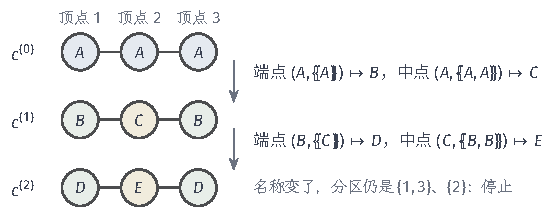
\includegraphics[width=94.0mm]{figures/01-basic-mathematics/04-graphs/tikz/c2-wl-path-refinement/figure.pdf}
  \caption{三点路径上的1-WL标记细化。每行是一轮标记，颜色表示所属的类；右侧是由签名得到新标记的编码。第一轮把端点与中点分开；第二轮标记名称改变，但划分仍为$\{1,3\}$、$\{2\}$，细化停止。}
  \label{fig:graph-trav-wl-path}
\end{figure}

\paragraph{只拆分不合并，有限轮后停止}
上例显示，判断停止要看划分，而不是看标记的名称。下面的引理说明划分只会越来越细，并且一旦某轮没有变化，以后也不会再变。

\begin{lemma}[1-WL的单调性与停止]
\label{lem:graph-trav-wl-refine}
对定义~\ref{def:graph-trav-wl-refinement}中的划分：（1）$\mathcal P^{(t+1)}$是$\mathcal P^{(t)}$的细分，即第$t+1$轮同类的顶点在第$t$轮也同类；（2）若$\mathcal P^{(t+1)}=\mathcal P^{(t)}$，则以后各轮划分都不再改变；（3）至多$n-1$轮严格细分后，划分就停止变化。
\end{lemma}

\begin{proof}
（1）若$c_i^{(t+1)}=c_j^{(t+1)}$，由$\operatorname{enc}$是单射得$\sigma_i^{(t)}=\sigma_j^{(t)}$，签名的第一个分量相等，即$c_i^{(t)}=c_j^{(t)}$。

（2）两轮划分相同，意味着存在标记之间的一一对应$\varphi$，使得对每个顶点$c_i^{(t+1)}=\varphi(c_i^{(t)})$。把$\varphi$作用到签名的每个分量上，得到$\sigma_i^{(t+1)}=\bigl(\varphi(c_i^{(t)}),\{\!\{\varphi(c_j^{(t)}):j\in N(i)\}\!\}\bigr)$。$\varphi$是一一对应，所以$\sigma_i^{(t+1)}=\sigma_k^{(t+1)}$当且仅当$\sigma_i^{(t)}=\sigma_k^{(t)}$，即$c_i^{(t+2)}=c_k^{(t+2)}$当且仅当$c_i^{(t+1)}=c_k^{(t+1)}$。因此$\mathcal P^{(t+2)}=\mathcal P^{(t+1)}$，依此类推。

（3）每次严格细分至少使类的个数加一，类的个数从至少$1$开始、不超过$n$，所以严格细分至多$n-1$次。由（2），第一次没有变化之后就再也不会变化。
\end{proof}

\paragraph{计算开销}
每一轮要为每个顶点读取全部邻居的标记，共$O(n+m)$次读取；把顶点$i$的邻居标记排序成多重集合的规范形式需要$O(d_i\log d_i)$时间；再把全部签名排序或查字典以分配新标记。一轮的总代价为$O((n+m)\log n)$量级。由引理~\ref{lem:graph-trav-wl-refine}，至多$n$轮就能确认划分稳定（最后一轮用于确认没有变化），所以总时间不超过$O(n(n+m)\log n)$。实际图上细化往往在少数几轮内稳定，总开销远小于这个上界。

\subsection{判别能力与局限}
\label{sec:graph-trav-wl-power}

\paragraph{在不交并上比较两个图}
要用1-WL比较图$\mathcal G_1$与$\mathcal G_2$，把两图放在一起看成一个不交并，用同一个初始标记规则和同一本字典同步细化，然后在每一轮分别统计两图中每种标记出现的次数。这种比较方法称为\term{一维Weisfeiler--Leman检验}（1-dimensional Weisfeiler--Leman test）。若某一轮两图的计数不同，就可以断定两图不同构；若计数在细化稳定前始终相同，只能说这一方法没有区分它们。

为什么计数不同就能断定不同构？设$\pi$是从$\mathcal G_1$到$\mathcal G_2$的同构，且初始标记满足$c_{\pi(i)}^{(0)}=c_i^{(0)}$（无属性时所有初始标记相同，自然满足；有属性时同构本来就要求保持属性）。$\pi$把$i$的邻居一一映为$\pi(i)$的邻居，对轮数归纳可得$\sigma_{\pi(i)}^{(t)}=\sigma_i^{(t)}$，于是$c_{\pi(i)}^{(t+1)}=c_i^{(t+1)}$。$\pi$是顶点之间的双射，每种标记在两图中的出现次数就相同。同样的推理说明，对同一个图重新编号顶点（用第~\ref{sec:graph-isomorphism}节的置换表示），各顶点的标记随之移动，标记计数不变：1-WL的结果不依赖编号，也不依赖图的画法。

例如，四个顶点的路径与四个顶点的星形都有$4$个顶点、$3$条边。初始标记全为$A$时，第一轮路径得到两个“一个邻居”的端点和两个“两个邻居”的内点，星形得到三个“一个邻居”的叶和一个“三个邻居”的中心，计数不同，两图不同构。这一轮区分的其实就是度分布，更多轮次则会区分邻居的度、邻居的邻居的度，等等。

\paragraph{六环与两个三角形}
1-WL的判别能力是有限的。图~\ref{fig:graph-trav-wl-limitation}中，六个顶点的环与两个不相连的三角形都有$6$个顶点、$6$条边，每个顶点的度都是$2$。初始标记全为$A$时，每个顶点的签名都是$(A,\{\!\{A,A\}\!\})$，所有顶点得到同一个新标记；下一轮又是同样的情形。标记从第一轮起就稳定为一类，两图的计数始终相同，1-WL无法区分它们。可是它们并不同构：六环是连通的，而两个三角形构成两个连通分量。用第~\ref{sec:graph-trav-components-forest}节的方法数一下连通分量，就能立刻把它们分开。

\begin{figure}[!htb]
  \centering
  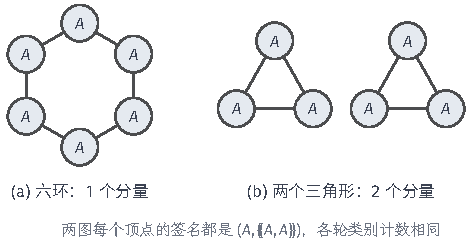
\includegraphics[width=79.5mm]{figures/01-basic-mathematics/04-graphs/tikz/c2-wl-cycle-triangles/figure.pdf}
  \caption{1-WL的局限。(a)六顶点环与(b)两个不相连的三角形初始标记全为$A$；每个顶点在每一轮都看到两个同类邻居，签名恒为$(A,\{\!\{A,A\}\!\})$，两图各轮的标记计数完全相同。两图分量数不同，并不同构。}
  \label{fig:graph-trav-wl-limitation}
\end{figure}

这个例子说明了1-WL的本质：每个顶点只能看到以自己为中心、逐轮向外扩大的邻域中“各类邻居有几个”，而六环和三角形上的每个顶点，无论看多少轮，看到的局部情形都一样。连通分量数这种整体性质，局部的计数无法反映。因此1-WL计数不同可以作为不同构的证据，计数相同则不能作为同构的证明。实践中常把它与分量数、环长等其他检验结合使用，各种检验互为补充；要确认同构，仍需给出一个实际的保持邻接的双射并逐边核对。
